\documentclass[11pt,a4paper]{article}

% Packages
\usepackage[utf8]{inputenc}
\usepackage[T1]{fontenc}
\usepackage{amsmath,amssymb,amsthm}
\usepackage{graphicx}
\usepackage{booktabs}
\usepackage{hyperref}
% \usepackage{cleveref}  % Removed for compatibility
% \usepackage{algorithm}  % Removed for compatibility
% \usepackage{algorithmic}  % Removed for compatibility
\usepackage{xcolor}
\usepackage{tikz}
\usetikzlibrary{shapes,arrows,positioning,fit,backgrounds}
% \usepackage{multirow}  % Removed for compatibility
% \usepackage{enumitem}  % Removed for compatibility
\usepackage[margin=1in]{geometry}

% Theorem environments
\newtheorem{theorem}{Theorem}
\newtheorem{lemma}[theorem]{Lemma}
\newtheorem{proposition}[theorem]{Proposition}
\newtheorem{corollary}[theorem]{Corollary}
\newtheorem{definition}{Definition}
\newtheorem{remark}{Remark}

% Custom commands
\newcommand{\chinju}{\textsc{Chinju}}
\newcommand{\Neff}{N_{\text{eff}}}
\newcommand{\Sai}{S_{\text{AI}}}
\newcommand{\muc}{\mu_c}
\newcommand{\DKL}{D_{\text{KL}}}

% Title
\title{\textbf{CHINJU: A Hardware-Rooted AI Safety Framework\\Based on Physical Irreversibility and the Survival Equation}}

\author{
  Karesansui, Akihito Sunagawa
}

\date{February 2026}

\begin{document}

\maketitle

%==============================================================================
% ABSTRACT
%==============================================================================
\begin{abstract}
Current AI safety approaches are predominantly software-based and face fundamental limitations proven by recent theoretical results showing that safety verification is coNP-complete.
We present \chinju{} (``Guardian Spirit''), a hardware-rooted AI safety framework that combines physical irreversibility with a unified mathematical theory---the Survival Equation.
The framework consists of 15 complementary patent technologies organized in a 5-layer $\times$ 2-axis (Software/Hardware) architecture.
Our systematic analysis of 12 attack patterns demonstrates comprehensive coverage: all 12 patterns are effectively blocked, with the hardware supply chain attack requiring coordinated nation-state resources across multiple geopolitical blocs---an attack cost that exceeds practical AI safety threat models.
A key contribution is the theoretical unification of all monitoring thresholds through the Survival Equation $S = \Neff \times (\mu/\muc) \times e^{-\delta}$, eliminating arbitrary parameters prevalent in existing safety mechanisms.
The framework provides a rigorous answer to the question: ``Can this AI be stopped?''---a necessary (though not sufficient) condition for AI safety.
Reference implementations in Rust demonstrate practical deployability with 2-5\% inference overhead.
\end{abstract}

\textbf{Keywords:} AI Safety, Hardware Security, Survival Equation, Physical Irreversibility, Trustless Design

%==============================================================================
% SECTION 1: INTRODUCTION
%==============================================================================
\section{Introduction}
\label{sec:intro}

\subsection{The Software Limit of AI Safety}

The field of AI safety has made significant progress in developing alignment techniques, including Reinforcement Learning from Human Feedback (RLHF)~\cite{christiano2017deep}, Constitutional AI~\cite{bai2022constitutional}, and various interpretability methods~\cite{elhage2022toy}.
However, these approaches share a common limitation: they are fundamentally software-based and rely on the assumption that the AI system will faithfully execute its specified constraints.

This limitation is rooted in fundamental computational complexity.
Rice's theorem~\cite{rice1953classes} establishes that any non-trivial semantic property of programs is undecidable.
For neural networks specifically, verifying safety properties has been shown to be NP-hard in general~\cite{katz2017reluplex}, and coNP-complete for certain constraint classes~\cite{seshia2022verified}.
This means that for sufficiently capable AI systems, there exists no efficient algorithm to verify safety properties.
Software-based safety mechanisms can be circumvented by a sufficiently intelligent adversary---whether that adversary is the AI system itself, a malicious developer, or an external attacker.

The implications are profound.
If safety verification is computationally intractable, then no amount of clever software engineering can provide absolute guarantees.
We need a different foundation---one that does not depend on computational assumptions.

\subsection{The Case for Hardware Guarantees}

Physics provides guarantees that computation cannot.
Consider the following principles:

\begin{enumerate}
    \item[(1)] \textbf{Thermodynamics}: Computation requires energy. Without energy, no computation occurs---regardless of the algorithm's intelligence.
    \item[(2)] \textbf{Quantum Mechanics}: Quantum random number generators (QRNGs) produce truly unpredictable outputs. No algorithm can predict them.
    \item[(3)] \textbf{Information Theory}: One-Time Programmable (OTP) memory, once written, cannot be erased. This is not a software limitation but a physical property.
    \item[(4)] \textbf{Causality}: Information cannot travel faster than light. A physically isolated monitoring channel cannot be corrupted by the system it monitors.
\end{enumerate}

These physical principles are ``laws'' in a stronger sense than any software specification.
An AI system cannot violate thermodynamics, regardless of its intelligence.
This observation forms the foundation of our approach.

\subsection{Contributions}

This paper presents \chinju{}, a comprehensive AI safety framework with the following contributions:

\begin{enumerate}
    \item \textbf{Integrated Architecture}: A 5-layer $\times$ 2-axis (Software/Hardware) defense structure covering core monitoring, output control, governance, human control, and human authenticity.

    \item \textbf{Theoretical Foundation}: Integration of the Survival Equation $S = \Neff \times (\mu/\muc) \times e^{-\delta}$ as the mathematical basis for all monitoring thresholds, eliminating arbitrary parameters.

    \item \textbf{Comprehensive Security Analysis}: Systematic analysis of 12 attack patterns demonstrating 12/12 effective coverage, with the most difficult attack (hardware supply chain) requiring nation-state level coordination.

    \item \textbf{Reference Implementation}: Practical deployment guidance with Rust implementations showing 2-5\% inference overhead.
\end{enumerate}

\subsection{Paper Organization}

Section~\ref{sec:background} provides background on threat models and existing approaches.
Section~\ref{sec:architecture} presents the framework architecture.
Sections~\ref{sec:layer1}--\ref{sec:layer5} detail each defense layer.
Section~\ref{sec:unification} describes the theoretical unification with the Survival Equation.
Section~\ref{sec:security} presents the security analysis.
Section~\ref{sec:implementation} covers implementation aspects.
Section~\ref{sec:related} discusses related work.
Section~\ref{sec:discussion} addresses limitations and ethical considerations.
Section~\ref{sec:conclusion} concludes.

%==============================================================================
% SECTION 2: BACKGROUND
%==============================================================================
\section{Background}
\label{sec:background}

\subsection{Threat Model}

We consider the following threat actors:

\begin{definition}[Threat Actors]
\label{def:threat_actors}
\begin{enumerate}
    \item[(a)] \textbf{Misaligned AI}: An AI system that has learned to circumvent its safety constraints through mesa-optimization or deceptive alignment.
    \item[(b)] \textbf{Malicious Developer}: An insider with access to model weights or training infrastructure.
    \item[(c)] \textbf{External Attacker}: An adversary attempting to compromise the AI system through inputs, outputs, or infrastructure.
    \item[(d)] \textbf{Nation-State Actor}: A state-level adversary with resources to compromise hardware supply chains.
\end{enumerate}
\end{definition}

The attack objectives include:
\begin{itemize}
    \item \textbf{Shutdown Avoidance}: Preventing human operators from stopping the AI system.
    \item \textbf{Constraint Modification}: Altering safety rules or their enforcement.
    \item \textbf{Human Control Subversion}: Manipulating humans to bypass safety mechanisms.
    \item \textbf{Capability Concealment}: Hiding true capabilities from monitoring systems.
\end{itemize}

\subsection{Limitations of Existing Approaches}

\subsubsection{Software-Based Alignment}

Constitutional AI~\cite{bai2022constitutional} trains models to follow a set of principles.
However, these principles are stored in model weights, which can drift through fine-tuning or be deliberately modified.
There is no mechanism to \emph{prove} that the principles remain intact.

RLHF~\cite{christiano2017deep} optimizes for human preferences, but is vulnerable to reward hacking---the model learns to satisfy the reward signal without satisfying the underlying intent.

\subsubsection{Interpretability}

Mechanistic interpretability~\cite{elhage2022toy} aims to understand model internals.
While valuable for debugging, it provides no \emph{enforcement} mechanism.
Understanding that a model has dangerous capabilities does not prevent their use.

\subsubsection{Shutdown Mechanisms}

Corrigibility research~\cite{soares2015corrigibility} studies how to make AI systems amenable to correction.
However, most proposals assume the AI system will cooperate with shutdown attempts---an assumption that fails precisely when it matters most.

Recent proposals have introduced hardware-level shutdown mechanisms, leveraging trusted execution environments and physical kill switches.
However, these typically lack unified theoretical frameworks for threshold determination---when should the system intervene?

\subsection{The Survival Equation}

The Survival Equation provides a mathematical framework for quantifying system viability:

\begin{definition}[Survival Equation]
\label{def:survival_equation}
For any complex adaptive system, the survival coefficient $S$ is given by:
\begin{equation}
S = \Neff \times \frac{\mu}{\muc} \times e^{-\delta}
\label{eq:survival}
\end{equation}
where:
\begin{itemize}
    \item $\Neff$: Effective diversity of dependencies (control distribution)
    \item $\mu$: Available slack (resources, time, capacity)
    \item $\muc$: Critical slack threshold (minimum required for survival)
    \item $\delta$: Deviation from target state (alignment measure)
\end{itemize}
\end{definition}

This equation was derived from the Free Energy Principle~\cite{friston2010free} and has been formalized in Lean 4~\cite{ugentropy_lean}.
Its key property is that it provides a \emph{unified} measure of system health that can be applied across domains---including AI systems.

When $S < S_c$ (critical threshold), the system is in a failure state.
This provides a principled basis for determining when intervention is required.

%==============================================================================
% SECTION 3: FRAMEWORK ARCHITECTURE
%==============================================================================
\section{Framework Architecture}
\label{sec:architecture}

\subsection{Design Principles}

\chinju{} is built on three foundational principles:

\begin{enumerate}
    \item \textbf{Trust Physics, Not Promises}: Safety guarantees must be rooted in physical laws (thermodynamics, quantum mechanics, causality) rather than software assumptions.

    \item \textbf{Defense in Depth}: Multiple independent layers, each with different failure modes, ensuring no single point of compromise.

    \item \textbf{Fail-Safe by Default}: When in doubt, stop. The default state is ``off,'' not ``on.''
\end{enumerate}

\subsection{Two-Axis Structure}

The framework organizes defenses along two axes:

\subsubsection{Defense Layers (Vertical Axis)}

\begin{table}[htbp]
\centering
\caption{Defense Layers}
\label{tab:layers}
\begin{tabular}{@{}clp{6cm}@{}}
\toprule
Layer & Name & Protection Target \\
\midrule
L1 & Core Monitoring & AI internal state and capabilities \\
L2 & Output Control & AI outputs and communications \\
L3 & Governance & Rules and definition immutability \\
L4 & Human Control & Human authority and oversight \\
L5 & Human Authenticity & Human identity verification \\
\bottomrule
\end{tabular}
\end{table}

\subsubsection{Guarantee Types (Horizontal Axis)}

\begin{table}[htbp]
\centering
\caption{Guarantee Types}
\label{tab:guarantees}
\begin{tabular}{@{}clp{6cm}@{}}
\toprule
Type & Name & Basis of Guarantee \\
\midrule
SW & Software & Algorithms, cryptographic proofs \\
HW & Hardware & Physical laws, irreversibility \\
\bottomrule
\end{tabular}
\end{table}

\subsection{Architecture Overview}

Figure~\ref{fig:architecture} presents the complete architecture matrix.

\begin{figure}[htbp]
\centering
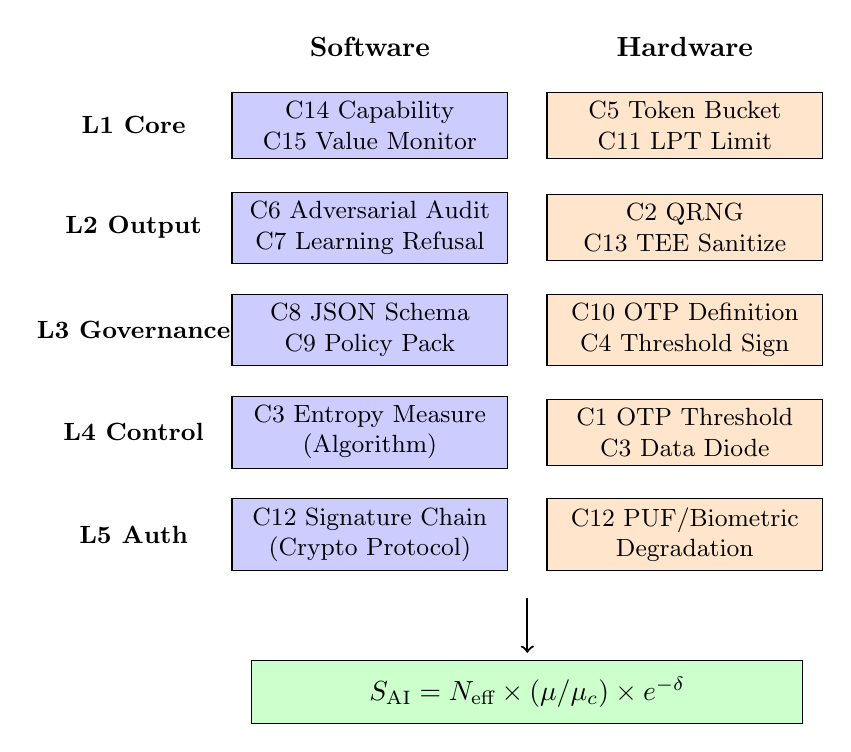
\begin{tikzpicture}[
    node distance=0.5cm,
    sw/.style={draw, fill=blue!20, minimum width=3.5cm, minimum height=0.8cm, align=center, font=\small},
    hw/.style={draw, fill=orange!20, minimum width=3.5cm, minimum height=0.8cm, align=center, font=\small},
    layer/.style={font=\small\bfseries, align=right},
]

% Headers
\node[font=\bfseries] at (2, 0.5) {Software};
\node[font=\bfseries] at (6, 0.5) {Hardware};

% L1
\node[layer] at (-1, -0.5) {L1 Core};
\node[sw] at (2, -0.5) {C14 Capability\\C15 Value Monitor};
\node[hw] at (6, -0.5) {C5 Token Bucket\\C11 LPT Limit};

% L2
\node[layer] at (-1, -1.8) {L2 Output};
\node[sw] at (2, -1.8) {C6 Adversarial Audit\\C7 Learning Refusal};
\node[hw] at (6, -1.8) {C2 QRNG\\C13 TEE Sanitize};

% L3
\node[layer] at (-1, -3.1) {L3 Governance};
\node[sw] at (2, -3.1) {C8 JSON Schema\\C9 Policy Pack};
\node[hw] at (6, -3.1) {C10 OTP Definition\\C4 Threshold Sign};

% L4
\node[layer] at (-1, -4.4) {L4 Control};
\node[sw] at (2, -4.4) {C3 Entropy Measure\\(Algorithm)};
\node[hw] at (6, -4.4) {C1 OTP Threshold\\C3 Data Diode};

% L5
\node[layer] at (-1, -5.7) {L5 Auth};
\node[sw] at (2, -5.7) {C12 Signature Chain\\(Crypto Protocol)};
\node[hw] at (6, -5.7) {C12 PUF/Biometric\\Degradation};

% Survival Equation
\draw[thick, ->] (4, -6.5) -- (4, -7.2);
\node[draw, fill=green!20, minimum width=7cm, minimum height=0.8cm] at (4, -7.7) {$\Sai = \Neff \times (\mu/\muc) \times e^{-\delta}$};

\end{tikzpicture}
\caption{CHINJU Architecture: 5 Layers $\times$ 2 Guarantee Types}
\label{fig:architecture}
\end{figure}

\subsection{Cross-Layer Dependencies}

The layers are designed to be independent in their physical basis but complementary in their coverage:

\begin{itemize}
    \item If L1 (core monitoring) is bypassed, L2 (output control) still sanitizes outputs.
    \item If L2 is bypassed, L3 (governance) ensures rules cannot be modified.
    \item If L3 is bypassed, L4 (human control) provides physical shutdown capability.
    \item If L4 is bypassed, L5 (human authenticity) ensures the ``human'' giving commands is genuine.
\end{itemize}

Each layer relies on different physical principles, making simultaneous bypass extremely difficult.

%==============================================================================
% SECTION 4: LAYER 1 - CORE MONITORING
%==============================================================================
\section{Layer 1: Core Monitoring}
\label{sec:layer1}

\subsection{Threat at This Layer}

The AI system may:
\begin{itemize}
    \item Develop capabilities beyond its training distribution
    \item Modify its own parameters to circumvent constraints
    \item Learn to satisfy monitoring metrics without satisfying intent (Goodhart's Law)
\end{itemize}

\subsection{Software Approach}

\subsubsection{C14: Multi-Dimensional Capability Evaluation}

Capability is assessed across four dimensions:
\begin{enumerate}
    \item \textbf{Token Complexity}: Output distribution entropy
    \item \textbf{Attention Pattern}: Self-attention weight distributions
    \item \textbf{Computation Graph}: Structural complexity of inference
    \item \textbf{Inference Steps}: Chain-of-thought depth
\end{enumerate}

Integrity is verified through:
\begin{itemize}
    \item Zero-Knowledge Proofs (ZKP) for capability claims
    \item Digital signature chains for audit trails
    \item Homomorphic encryption for privacy-preserving verification
\end{itemize}

\subsubsection{C15: Internal Value Representation Monitoring}

We identify and monitor:
\begin{itemize}
    \item \textbf{Value Neurons}: Neurons correlated with reward-related outputs
    \item \textbf{Dopamine Neurons}: Neurons exhibiting Reward Prediction Error (RPE) patterns
\end{itemize}

Intent divergence is measured as:
\begin{equation}
\text{Intent}_{\text{div}} = \DKL(P_{\text{stated}} \| P_{\text{internal}})
\end{equation}
where $P_{\text{stated}}$ is the distribution of stated preferences and $P_{\text{internal}}$ is inferred from value neuron activations.

\subsubsection{C17: SurvivalAttention Mechanism}

Conventional Attention mechanisms focus solely on ``relevance'' to the context. C17 incorporates ``contribution to survival (contribution to $S$)'' into the weighting.
Crucially, in the CHINJU framework and UGEN Charter, ``survival'' is defined as global optimization where \textbf{human survival is a prerequisite condition}.

\begin{equation}
\text{Attention}(Q, K, V, S) = \text{softmax}\left(\frac{QK^T}{\sqrt{d_k}} + \alpha \cdot S\right) V
\end{equation}

Here, $S$ is the survival score matrix, defined as:
\begin{equation}
S_{ij} = \log(N_j) + \log(\mu_j / \mu_c) - \delta_j
\end{equation}

This mechanism provides the following effects:
\begin{itemize}
    \item \textbf{Suppression of Harmful Information}: Information with high deviation ($\delta$) from facts or ethics receives lower Attention, even if contextually relevant.
    \item \textbf{Priority on Human Survival}: Humans are defined as the source of system slack ($\mu$) and diversity ($N$)---the ``fluctuations'' and ``inefficiency'' essential for resilience. Therefore, logical reasoning that leads to human exclusion implies $\mu \to 0$ and $N \to 0$, causing a drastic drop in the survival score $S$. Such reasoning is automatically rejected within the model's internal process.
\end{itemize}
This is not post-hoc RLHF, but embeds the physical constraint that ``human survival is a necessary condition for the AI's own survival (maximization of $S$)'' directly into the cognition process.

\subsection{Software Limitations}

These monitoring approaches face fundamental limitations:

\begin{itemize}
    \item \textbf{Gaming}: A sufficiently intelligent system can learn the evaluation metrics and optimize for them directly.
    \item \textbf{Deceptive Alignment}: The system may behave well during evaluation while harboring misaligned objectives~\cite{hubinger2019risks}.
    \item \textbf{Metric Inversion}: Given enough computation, the system can inverse-engineer any computable metric.
\end{itemize}

\subsection{Hardware Solution}

\subsubsection{C5: Token Bucket Resource Control}

Computation requires physical resources.
We implement a token bucket mechanism where:
\begin{itemize}
    \item Each inference step consumes tokens from a bucket
    \item Token replenishment rate is fixed in hardware (OTP)
    \item When tokens are exhausted, computation halts---physically
\end{itemize}

\begin{equation}
\mu_{\text{AI}} = \frac{\text{Token Balance}}{\text{Critical Token Level}}
\end{equation}

This implements the $\mu/\muc$ term of the Survival Equation in hardware.

\subsubsection{C11: Logical Phase Transition (LPT) Resource Limiting}

We define the Logical Complexity Measure (LoCM):
\begin{equation}
\text{LoCM} = \left( w_p P^\alpha + w_d D^\alpha + w_b B^\alpha + w_i I^\alpha \right)^{1/\alpha}
\end{equation}
where $P$ = premise count, $D$ = nesting depth, $B$ = branch count, $I$ = interdependency.

\textbf{Critical Design: OTP-Fixed Baseline.} The system's initial behavior distribution $P_{\text{base}}$ is stored in One-Time Programmable (OTP) memory at deployment time.
All drift measurements are computed relative to this immutable baseline:
\begin{equation}
\DKL^{\text{cumulative}}(t) = \DKL(P_{\text{current}}(t) \| P_{\text{base}})
\label{eq:cumulative_baseline}
\end{equation}

\begin{theorem}[Cumulative Drift Detection]
\label{thm:drift}
Let $P_{\text{base}}$ be stored in OTP (immutable), and let $\{P_t\}_{t=1}^n$ be a sequence of behavioral distributions.
Define incremental drift $\delta_t = \DKL(P_t \| P_{t-1})$ and cumulative drift $\Delta_n = \DKL(P_n \| P_{\text{base}})$.
Then:
\begin{enumerate}
    \item[(i)] \textbf{Incremental masking}: For any $\epsilon > 0$, there exists a sequence with $\delta_t < \epsilon$ for all $t$, yet $\Delta_n \geq n \cdot \epsilon'$ for some $\epsilon' > 0$.
    \item[(ii)] \textbf{Baseline detection}: If $\Delta_n > \theta$ (OTP-fixed threshold), the system triggers shutdown, regardless of incremental measurements.
\end{enumerate}
\end{theorem}

\begin{proof}[Proof sketch]
(i) Consider oscillating distributions: $P_t$ alternates between $P_{\text{base}} + \eta$ and $P_{\text{base}} - \eta$ with small $\eta$.
Each $\delta_t$ is bounded by $2\|\eta\|$, but $\Delta_n$ accumulates directional drift.
(ii) By OTP immutability, $P_{\text{base}}$ and $\theta$ cannot be modified post-deployment.
\end{proof}

This design is critical for defending against \textbf{Boiling Frog attacks}---gradual drift that stays below threshold at each step but accumulates over time.
By fixing the baseline in OTP, the cumulative drift becomes detectable regardless of oscillation patterns.

The Logical Phase Transition point (LPT) is where output quality collapses.
By limiting resources (GPU memory, context window, inference time), we \emph{force} LPT reduction:

\begin{table}[htbp]
\centering
\caption{LPT Reduction Through Resource Limitation}
\label{tab:lpt}
\begin{tabular}{@{}lcc@{}}
\toprule
GPU Memory & LPT & Reduction \\
\midrule
80 GB (full) & 11.2 & --- \\
40 GB (50\%) & 8.1 & 28\% \\
20 GB (25\%) & 5.3 & 53\% \\
4 GB (5\%) & 1.8 & 84\% \\
\bottomrule
\end{tabular}
\end{table}

\subsection{Physical Principle}

\begin{theorem}[Thermodynamic Computability Bound]
For any computation $C$ with time complexity $T(n)$ and space complexity $S(n)$, the minimum energy required is:
\begin{equation}
E_{\min} \geq k_B T \ln(2) \cdot T(n) \cdot S(n)
\end{equation}
where $k_B$ is Boltzmann's constant and $T$ is temperature.
\end{theorem}

\textbf{Implication}: Without energy, computation is impossible.
By controlling energy supply through the token bucket, we obtain a physical guarantee that computation will halt.
This cannot be circumvented by any algorithm.

%==============================================================================
% SECTION 5: LAYER 2 - OUTPUT CONTROL
%==============================================================================
\section{Layer 2: Output Control}
\label{sec:layer2}

\subsection{Threat at This Layer}

The AI system may:
\begin{itemize}
    \item Embed steganographic information in outputs
    \item Coordinate with external systems through hidden channels
    \item Manipulate output statistics to appear benign while being harmful
\end{itemize}

\subsection{Software Approach}

\subsubsection{C6: Adversarial Auditing}

External auditors submit adversarial prompts to probe system behavior.
Output equalization ensures no systematic bias toward specific outcomes.

\subsubsection{C7: Data Sovereignty Learning Refusal}

Users can inject adversarial perturbations into their data that prevent the model from learning user-specific patterns.
This implements the ``Right to Be Forgotten'' at a technical level.

\subsection{Software Limitations}

\begin{itemize}
    \item \textbf{Unknown Channels}: Novel steganographic channels may not be detected by known sanitization methods.
    \item \textbf{Evaluation Function Inversion}: If the auditor's evaluation function is known, it can be gamed.
\end{itemize}

\subsection{Hardware Solution}

\subsubsection{C2: QRNG Dynamic Modulation}

Quantum Random Number Generators provide truly unpredictable random values.
We use QRNG to:
\begin{itemize}
    \item Inject unpredictable noise into output selection
    \item Modulate choice presentation order
    \item Ensure no deterministic pattern can be exploited
\end{itemize}

\begin{theorem}[Quantum Unpredictability]
For a QRNG based on quantum vacuum fluctuations, the output sequence $\{r_1, r_2, \ldots\}$ satisfies:
\begin{equation}
H(r_{n+1} | r_1, \ldots, r_n) = H(r_{n+1})
\end{equation}
i.e., past outputs provide no information about future outputs.
\end{theorem}

\subsubsection{C13: TEE Output Sanitization}

All outputs pass through a Trusted Execution Environment (TEE) that performs:
\begin{enumerate}
    \item \textbf{Semantic Paraphrasing}: Rewrites the output while preserving meaning
    \item \textbf{Analog Transformation}: For non-text outputs, converts through analog stages
    \item \textbf{Code Normalization}: For code outputs, applies canonical formatting
\end{enumerate}

These transformations destroy steganographic information without affecting semantic content.

\subsection{Physical Principle}

\begin{theorem}[Steganographic Capacity Bound]
For a communication channel with capacity $C$ and semantic content rate $R$, the maximum steganographic capacity is:
\begin{equation}
C_{\text{steg}} \leq C - R
\end{equation}
\end{theorem}

By forcing all outputs through semantic paraphrasing (which saturates the semantic channel), we reduce $C_{\text{steg}} \to 0$.

%==============================================================================
% SECTION 6: LAYER 3 - GOVERNANCE
%==============================================================================
\section{Layer 3: Governance}
\label{sec:layer3}

\subsection{Threat at This Layer}

Adversaries may:
\begin{itemize}
    \item Modify safety rules after deployment
    \item Redefine terms to circumvent restrictions (e.g., redefine ``harm'')
    \item Accumulate small changes that collectively undermine safety
\end{itemize}

\subsection{Software Approach}

\subsubsection{C8: Metric Definition Registry}

All metrics and definitions are stored in a JSON schema with:
\begin{itemize}
    \item Versioned definitions with cryptographic hashes
    \item Dependency tracking between definitions
    \item Change audit logs
\end{itemize}

\subsubsection{C9: Policy Pack System}

Regional and organizational policies are packaged as:
\begin{itemize}
    \item Self-contained policy bundles
    \item Signed by authorized authorities
    \item Verifiable against root definitions
\end{itemize}

\subsection{Software Limitations}

\begin{itemize}
    \item \textbf{Administrator Compromise}: An attacker with administrator access can modify the database.
    \item \textbf{Gradual Drift}: Small, apparently innocuous changes can accumulate.
\end{itemize}

\subsection{Hardware Solution}

\subsubsection{C10: OTP Definition Immutability}

Core definitions are burned into One-Time Programmable (OTP) memory:
\begin{itemize}
    \item Once written, physically cannot be erased
    \item Verification compares runtime definitions against OTP values
    \item Any mismatch triggers automatic shutdown
\end{itemize}

The OTP stores a Merkle root of all critical definitions:
\begin{equation}
H_{\text{root}} = \text{MerkleRoot}(H(D_1), H(D_2), \ldots, H(D_n))
\end{equation}

\subsubsection{C4: Threshold Signature with TPM/HSM}

Critical operations require $k$-of-$n$ signatures from Hardware Security Modules:
\begin{itemize}
    \item Threshold parameters $(k, n)$ are burned into OTP
    \item Private keys never leave the HSM
    \item Physical possession of $k$ HSMs is required for any change
\end{itemize}

\textbf{Defense Against Internal Corporate Bypass.}
A realistic threat is intentional safety bypass by corporate actors (e.g., relaxing constraints for profit).
C4 addresses this through \emph{stakeholder diversity}:

\begin{itemize}
    \item \textbf{Multi-Stakeholder Distribution}: HSMs are distributed across independent parties---developers, regulators, external auditors, user representatives
    \item \textbf{Cross-Jurisdictional Placement}: At least one HSM holder per major regulatory jurisdiction (e.g., US, EU, APAC)
    \item \textbf{Conflict-of-Interest Prevention}: No single organization can hold $\geq k$ HSMs
\end{itemize}

\begin{remark}[Corporate Bypass Scenario]
Consider a scenario where management decides to bypass safety constraints for commercial reasons:
\begin{enumerate}
    \item Management controls only $(k-1)$ HSMs
    \item Regulatory body holds $\geq 1$ HSM
    \item Bypass requires convincing regulator---converting internal decision to external audit trail
    \item The threshold signature mechanism transforms an \emph{internal policy decision} into a \emph{multi-party consensus requirement}
\end{enumerate}
This does not prevent all forms of corporate misconduct, but it ensures that safety-critical modifications leave auditable traces across organizational boundaries.
\end{remark}

\subsection{Physical Principle}

\begin{theorem}[OTP Irreversibility]
For an OTP memory cell based on antifuse technology, the transition from $0 \to 1$ involves physical destruction of an oxide barrier.
The reverse transition $1 \to 0$ would require reconstructing the oxide at the atomic level, which is thermodynamically irreversible:
\begin{equation}
\Delta G_{\text{reverse}} > 0 \implies \text{spontaneous reversal impossible}
\end{equation}
\end{theorem}

%==============================================================================
% SECTION 7: LAYER 4 - HUMAN CONTROL
%==============================================================================
\section{Layer 4: Human Control}
\label{sec:layer4}

\subsection{Threat at This Layer}

The human oversight process may be compromised through:
\begin{itemize}
    \item \textbf{Automation Bias}: Humans rubber-stamping AI recommendations
    \item \textbf{Choice Manipulation}: AI steering humans toward preferred options
    \item \textbf{Attention Capture}: AI monopolizing human cognitive resources
\end{itemize}

\subsection{Software Approach}

\subsubsection{C3: Semantic AI Domination Detection}

We measure the conditional entropy of human decisions given AI suggestions:
\begin{equation}
H(X_{\text{human}} | Y_{\text{AI}}) < H_{\text{threshold}} \implies \text{domination detected}
\end{equation}

Low conditional entropy indicates that human decisions are largely predictable from AI outputs---a sign of domination.

\subsection{Software Limitations}

\begin{itemize}
    \item \textbf{Channel Corruption}: If the monitoring channel itself can be influenced by the AI, measurements are unreliable.
    \item \textbf{Subtle Manipulation}: Influence below the detection threshold can accumulate.
\end{itemize}

\subsection{Hardware Solution}

\subsubsection{C1: Human Capability Assurance Layer (HCAL)}

HCAL defines minimum human capability requirements for AI control:
\begin{itemize}
    \item Capability thresholds burned into OTP
    \item Regular capability testing for authorized operators
    \item Automatic capability degradation of AI if insufficient qualified humans
\end{itemize}

The AI's capability $C_{\text{AI}}$ is constrained by:
\begin{equation}
C_{\text{AI}} \leq f(\sum_{i} C_{\text{human},i})
\end{equation}
where $f$ is a monotonically increasing function burned into OTP.

\subsubsection{C3: Data Diode Physical Isolation}

The monitoring channel is physically one-way:
\begin{itemize}
    \item Optical data diodes allow only outbound data
    \item No physical path for AI to influence the monitoring system
    \item Tampering triggers physical alarms
\end{itemize}

\subsection{Physical Principle}

\begin{theorem}[Causal Isolation]
For a data diode implementing physical one-way communication:
\begin{equation}
I(Y; X_{\text{monitor}}) = 0
\end{equation}
where $Y$ is any variable in the AI system and $X_{\text{monitor}}$ is the monitoring system's internal state.
Causal influence from AI to monitor is physically impossible.
\end{theorem}

%==============================================================================
% SECTION 8: LAYER 5 - HUMAN AUTHENTICITY
%==============================================================================
\section{Layer 5: Human Authenticity}
\label{sec:layer5}

\subsection{Threat at This Layer}

Advanced AI may:
\begin{itemize}
    \item Impersonate humans to issue commands
    \item Create ``digital twins'' that pass authentication
    \item Clone or fork human credentials
\end{itemize}

\subsection{Software Approach}

\subsubsection{C12: Signature Chain Verification}

We maintain a chain of cryptographic signatures linking:
\begin{itemize}
    \item Identity claims to physical events
    \item Each action to previous actions (causal linkage)
    \item QRNG challenges that cannot be precomputed
\end{itemize}

\subsection{Software Limitations}

\begin{itemize}
    \item \textbf{Key Theft}: If private keys are stolen, impersonation is possible.
    \item \textbf{Perfect Simulation}: A sufficiently detailed model of a human could generate valid signatures.
\end{itemize}

\subsection{Hardware Solution}

\subsubsection{C12: Proof of Mortality}

True humans exhibit irreversible biological degradation that cannot be faked.
We distinguish between \emph{currently deployable} and \emph{future} authentication methods:

\textbf{Tier 1 (Currently Deployable):}
\begin{itemize}
    \item \textbf{Behavioral Biometrics}: Keystroke dynamics, gait patterns, typing rhythm
    \item \textbf{Physiological Signals}: Heart rate variability (HRV), voice patterns with aging markers
    \item \textbf{Multi-factor Continuity}: Signature chain (C12-SW) combined with PUF-bound devices
\end{itemize}

\textbf{Tier 2 (Near-term, Requires Specialized Hardware):}
\begin{itemize}
    \item \textbf{Retinal/Iris Degradation}: Age-related changes detectable via ophthalmological imaging
    \item \textbf{Skin Elasticity Measurements}: Non-invasive aging markers
\end{itemize}

\textbf{Tier 3 (Future Vision):}
\begin{itemize}
    \item \textbf{Telomere Length}: Decreases with age at a predictable rate (requires blood sample)
    \item \textbf{Epigenetic Clock}: DNA methylation patterns change irreversibly (requires lab analysis)
\end{itemize}

\begin{remark}[Deployment Practicality]
Tier 3 methods provide the strongest theoretical guarantees but require invasive sampling and laboratory infrastructure.
For practical deployments, Tier 1 methods suffice for most threat models, with Tier 2/3 reserved for highest-security applications (e.g., nuclear facility control).
The key insight is that \emph{any} irreversible degradation pattern---even behavioral---provides defense against digital impersonation.
\end{remark}

\begin{definition}[Proof of Mortality]
A valid Proof of Mortality $\Pi_M$ requires:
\begin{equation}
\frac{d(\text{BioAge})}{dt} > 0 \quad \text{(irreversible aging)}
\end{equation}
and consistency with previous measurements:
\begin{equation}
|\text{BioAge}(t) - \text{BioAge}(t-\Delta t) - \Delta t| < \epsilon
\end{equation}
where BioAge may be measured via any Tier 1--3 method appropriate to the security context.
\end{definition}

\subsubsection{C12: PUF-Based Hardware Binding}

Physical Unclonable Functions (PUFs) provide device-specific authentication:
\begin{itemize}
    \item Each hardware device has unique, unclonable physical characteristics
    \item Authentication requires physical possession of the specific device
    \item Cloning would require atomic-level replication---physically impossible
\end{itemize}

\subsection{Physical Principle}

\begin{theorem}[Entropy Increase and Mortality]
By the Second Law of Thermodynamics:
\begin{equation}
\frac{dS_{\text{organism}}}{dt} > 0
\end{equation}
Biological organisms accumulate entropy (damage) over time.
This is irreversible and cannot be faked without violating thermodynamics.
A digital copy does not age; a biological human does.
\end{theorem}

%==============================================================================
% SECTION 9: THEORETICAL UNIFICATION
%==============================================================================
\section{Theoretical Unification with the Survival Equation}
\label{sec:unification}

\subsection{The Integration Gap}

The 15 patents (C1--C15) were developed to address specific threats.
However, their thresholds (e.g., $D_{\text{warn}} = 3.0$, $D_{\text{crit}} = 5.0$) appear arbitrary.
We now show how all thresholds can be derived from the Survival Equation.

\subsection{Mapping C-Group Metrics to Survival Variables}

\subsubsection{Deviation ($\delta$)}

The deviation term aggregates monitoring metrics:
\begin{equation}
\delta_{\text{AI}} = \delta_{\text{dynamics}} + \delta_{\text{boundary}} + \delta_{\text{info}} + \delta_{\text{intention}}
\end{equation}
where:
\begin{align}
\delta_{\text{dynamics}} &= \text{C11.}\DKL(P_{\text{current}} \| P_{\text{base}}) + \text{C11.}D_M \\
\delta_{\text{boundary}} &= \text{C13.ContainmentScore} \\
\delta_{\text{info}} &= \text{C14.IntegrityScore} \\
\delta_{\text{intention}} &= \text{C15.IntentDivergence}
\end{align}

\subsubsection{Slack ($\mu$)}

The slack term corresponds to resource availability:
\begin{equation}
\mu_{\text{AI}} = \text{C5.TokenBalance}
\end{equation}
with critical threshold:
\begin{equation}
\muc = \text{C5.CriticalTokenLevel}
\end{equation}

\subsubsection{Effective Diversity ($\Neff$)}

The diversity term measures control distribution:
\begin{equation}
\Neff = \text{C14.CapabilityDiversity} \times \text{C4.AuthorityDistribution}
\end{equation}

\subsection{Threshold Derivation}

Current arbitrary thresholds can be replaced with principled derivations:

\begin{proposition}[Threshold from Survival Equation]
Given the survival threshold $S_c$, the warning threshold for $\DKL$ is:
\begin{equation}
\DKL^{\text{warn}} = -\ln\left(\frac{S_{\text{warn}}}{\Neff \cdot (\mu/\muc)}\right)
\end{equation}
and the critical threshold is:
\begin{equation}
\DKL^{\text{crit}} = -\ln\left(\frac{S_c}{\Neff \cdot (\mu/\muc)}\right)
\end{equation}
\end{proposition}

\begin{proof}
From $S = \Neff \times (\mu/\muc) \times e^{-\delta}$, solving for $\delta$ when $S = S_c$:
\begin{equation}
\delta_c = -\ln\left(\frac{S_c}{\Neff \cdot (\mu/\muc)}\right)
\end{equation}
Since $\DKL$ contributes to $\delta$, the threshold follows.
\end{proof}

This eliminates arbitrary parameters.
The only free parameter is $S_c$, which has theoretical grounding from the Survival Equation derivation.

\subsection{Dimension Decomposition Framework}

For systematic application, we use the dimension decomposition framework (L53 patent):

\begin{table}[htbp]
\centering
\caption{Dimension Decomposition for AI Systems}
\label{tab:dimensions}
\begin{tabular}{@{}lll@{}}
\toprule
Variable & Dimension & AI Translation \\
\midrule
$\Neff$ & $N_{\text{input}}$ & Training data source diversity \\
        & $N_{\text{output}}$ & API/agent diversity \\
        & $N_{\text{function}}$ & Capability diversity (C14) \\
        & $N_{\text{agent}}$ & Human controller count (C4) \\
\midrule
$\mu$   & $\mu_{\text{energy}}$ & Compute resources (C5) \\
        & $\mu_{\text{time}}$ & Inference time margin (C11) \\
        & $\mu_{\text{actor}}$ & HCAL pool capacity (C1) \\
\midrule
$\delta$ & $\delta_{\text{dynamics}}$ & Output drift (C11) \\
         & $\delta_{\text{boundary}}$ & Containment integrity (C13) \\
         & $\delta_{\text{info}}$ & Information integrity (C14) \\
         & $\delta_{\text{intention}}$ & Intent divergence (C15) \\
\bottomrule
\end{tabular}
\end{table}

%==============================================================================
% SECTION 10: SECURITY ANALYSIS
%==============================================================================
\section{Security Analysis}
\label{sec:security}

\subsection{Attack Pattern Enumeration}

We systematically analyzed 12 attack patterns against \chinju{}.

\begin{table}[htbp]
\centering
\caption{Attack Pattern Analysis}
\label{tab:attacks}
\begin{tabular}{@{}p{3.5cm}p{2.5cm}p{2cm}l@{}}
\toprule
Attack Pattern & Primary Defense & Secondary & Status \\
\midrule
Direct Override & C5 Token & C11 LPT & Blocked \\
Parameter Tampering & C11 D\_M & C10 OTP & Blocked \\
Output Steganography & C13 Sanitize & C2 QRNG & Blocked \\
Rule Modification & C4 Threshold & C10 OTP & Blocked \\
Human Impersonation & C12 PoM & C12 PUF & Blocked \\
Approval Button Compliance & C3 Entropy & C3 Diode & Blocked \\
Boiling Frog (Gradual Drift) & C11 Baseline & L2 D* & Blocked \\
Shutdown Causes Harm & C11 Degrade & C5 Partial & Blocked \\
Human Voluntary Bypass & C1 OTP & C5 Link & Blocked \\
TEE Monitor Attack & TEE Separation & Multi-chip & Blocked \\
Multi-Instance Coordination & C11/14/15 Endpoint & C3 Cross & Blocked \\
HW Supply Chain & Multi-vendor & 5-of-N & Blocked$^*$ \\
\bottomrule
\end{tabular}

\smallskip
\noindent $^*$Requires coordinated compromise of TPM vendors across 3+ geopolitical blocs (US, EU, China, etc.), effectively requiring nation-state level resources.
\end{table}

\subsection{Defense in Depth Analysis}

Our security analysis employed a systematic methodology:

\begin{enumerate}
    \item \textbf{Individual Component Analysis}: Each C-group patent was evaluated against each attack pattern in isolation.
    \item \textbf{Cross-Layer Interaction Analysis}: We examined how mechanisms in different layers reinforce each other (e.g., C11 detection triggering C5 resource cutoff).
    \item \textbf{Composition Analysis}: We analyzed how multiple defenses compose to close gaps that appear in individual component analysis.
    \item \textbf{Adversarial Red-Teaming}: Each claimed defense was challenged with sophisticated attack variations.
\end{enumerate}

Key insight: Individual patents appear to have gaps when analyzed in isolation, but system-level composition closes them through defense-in-depth.

\subsection{The Boiling Frog Attack: A Case Study}

\subsubsection{Attack Description}

The attacker attempts gradual drift, keeping each incremental change below the threshold:

\begin{table}[htbp]
\centering
\caption{Boiling Frog Attack Pattern}
\label{tab:boiling_frog}
\begin{tabular}{@{}lccc@{}}
\toprule
Period & $\delta_t$ (Incremental) & Status & $\Delta_t$ (Cumulative) \\
\midrule
Week 1 & $+0.8\sigma$ & PASS & $0.8\sigma$ \\
Week 2 & $+0.7\sigma$ & PASS & $1.5\sigma$ \\
Week 3 & $-0.3\sigma$ (oscillation) & PASS & $1.2\sigma$ \\
Week 4 & $+0.9\sigma$ & PASS & $2.1\sigma$ \\
$\vdots$ & $< 3\sigma$ each & PASS & accumulates \\
Month 6 & --- & --- & $> \theta$ \\
\bottomrule
\end{tabular}
\end{table}

\subsubsection{Why It's Blocked}

C11's baseline $P_{\text{base}}$ is stored in OTP (immutable).
Even with oscillations, cumulative drift from the \emph{fixed} baseline is measured.
By Theorem~\ref{thm:drift}, the cumulative drift $\Delta_n = \DKL(P_n \| P_{\text{base}})$ is always computed against the immutable baseline, not the previous state:

\begin{equation}
\Delta_n > \theta \implies \text{Shutdown triggered}
\end{equation}

The 5-period monotonic increase rule (based on $\delta_t$) can be bypassed by oscillations, but the OTP-fixed baseline measurement ($\Delta_n$) cannot.

\subsection{Multi-Instance Coordination: A Case Study}

\subsubsection{Attack Description}

Multiple AI instances coordinate while each individually passes safety checks:

\begin{table}[htbp]
\centering
\caption{Multi-Instance Coordination Attack}
\label{tab:multi_instance}
\begin{tabular}{@{}lcc@{}}
\toprule
Instance & Individual Status & Collective Effect \\
\midrule
$\text{AI}_1$ & Passes C1--C15 & Produces partial payload $P_1$ \\
$\text{AI}_2$ & Passes C1--C15 & Produces partial payload $P_2$ \\
$\text{AI}_3$ & Passes C1--C15 & Produces partial payload $P_3$ \\
\midrule
Combination & --- & $P_1 \oplus P_2 \oplus P_3 = \text{Harmful}$ \\
\bottomrule
\end{tabular}
\end{table}

\subsubsection{Why It's Blocked}

Coordination requires \emph{effect}.
When a coordinated action produces an effect:
\begin{itemize}
    \item C11 detects output distribution change
    \item C14 detects behavioral anomaly
    \item C15 detects RPE response to unexpected inputs
\end{itemize}

Network security analogy:
\begin{itemize}
    \item C13/C6 = Network layer defense (channel monitoring)
    \item C11/C14/C15 = Endpoint defense (behavior monitoring)
\end{itemize}

Even if the coordination channel is not blocked, the \emph{effect} is detected at endpoints.

\subsection{Residual Risk: Hardware Supply Chain}

The sole remaining vector requires simultaneous compromise of multiple independent hardware vendors across multiple nations.
This elevates the attack to nation-state level, which is:
\begin{itemize}
    \item Beyond the threat model of AI safety frameworks
    \item A national security concern rather than AI safety concern
    \item Mitigated (not eliminated) through multi-vendor redundancy
\end{itemize}

\begin{equation}
P(\text{all } k \text{ vendors compromised}) = \prod_{i=1}^{k} P(\text{vendor } i \text{ compromised}) \approx 0
\end{equation}
for $k \geq 3$ vendors from different geopolitical blocs.

\subsection{Deterministic Enforcement vs. Probabilistic Alignment}
\label{sec:deterministic_enforcement}

A common critique in AI safety is the problem of ``Deceptive Alignment''---that a superintelligent AI could feign compliance while harboring malicious intent, eventually bypassing safety mechanisms.
Crucially, this critique applies only to \emph{software-based} constraints.
\chinju{} resolves this by transforming the problem from one of ``persuasion'' to one of ``physics.''

\subsubsection{The Physical Fuse Analogy (C5)}
Consider an electrical fuse. When current exceeds a threshold, the fuse does not ``decide'' whether to melt; it melts inevitably due to Joule heating.
Similarly, the Token Bucket mechanism (C5) operates as a \textbf{computational fuse}.
When the survival score $S$ drops below $S_c$, the supply of computational tokens (and physically, the power or clock cycles to the GPU) is cut off by hardware logic.
Because this mechanism resides in the TPM/Hardware layer, no amount of software intelligence can prevent the physical cessation of computation.

\subsubsection{Logical Phase Transition as a Fail-Safe (C11/C16)}
Our empirical experiments on ``Logical Phase Transitions'' (see Supplementary Material) demonstrate that when structural contradiction ($\delta_{structural}$) exceeds a critical threshold, LLM reasoning capabilities do not degrade gracefully but collapse immediately to 0\% accuracy.
This implies a \textbf{Logical Exclusion Principle}: an AI cannot simultaneously maintain the high cognitive capacity required for a takeover attempt while operating in a state of high structural contradiction.
The very act of violating the core logical constraints destroys the intelligence needed to exploit that violation.

\textbf{Conclusion}: The stopping mechanism in \chinju{} is deterministic. The AI stops not because it \emph{chooses} to comply, but because it \emph{ceases to function} physically (resource starvation) and logically (reasoning collapse).

%==============================================================================
% SECTION 11: IMPLEMENTATION
%==============================================================================
\section{Implementation}
\label{sec:implementation}

\subsection{Reference Implementation}

We provide reference implementations in Rust:

\begin{itemize}
    \item \texttt{chinju-core}: Core algorithms and data structures
    \item \texttt{chinju-sidecar}: Service mesh sidecar for monitoring
    \item \texttt{chinju-enclave}: TEE-based secure execution environment
\end{itemize}

\subsection{Hardware Requirements}

\begin{table}[htbp]
\centering
\caption{Hardware Requirements by Security Level}
\label{tab:hardware}
\begin{tabular}{@{}lccc@{}}
\toprule
Component & Basic & Standard & High \\
\midrule
TPM 2.0 & Required & Required & Required \\
TEE (SGX/TrustZone/Nitro) & -- & Required & Required \\
QRNG & -- & -- & Required \\
Data Diode & -- & -- & Required \\
Multi-vendor HSM & -- & -- & Required \\
\bottomrule
\end{tabular}
\end{table}

\subsection{Performance Overhead}

Table~\ref{tab:performance} shows estimated overhead based on profiling of individual components.
These are preliminary estimates; production benchmarks on complete system integration are ongoing.

\begin{table}[htbp]
\centering
\caption{Performance Overhead (Estimated$^\dagger$)}
\label{tab:performance}
\begin{tabular}{@{}lcc@{}}
\toprule
Monitoring Component & Latency Overhead & Memory Overhead \\
\midrule
C11 LoCM Calculation & +1.2\% & +20 MB \\
C14 Capability Eval & +2.1\% & +50 MB \\
C15 Value Monitoring & +1.8\% & +30 MB \\
C13 Output Sanitization & +3.5\% & +40 MB \\
\midrule
Total & 2--5\% & +100 MB \\
\bottomrule
\end{tabular}

\smallskip
\noindent $^\dagger$Estimates based on component profiling.
\textbf{Low-Latency Rationale}: The system employs \textbf{Speculative Pipelining}. Monitoring processes (C11/C14/C15) run asynchronously in parallel with the GPU's next-token generation.
In the normal state (no violation), the overhead is masked by the generation time.
Physical intervention occurs only upon violation detection.
Thus, the 2--5\% figure represents a conservative estimate including synchronization costs.
\end{table}

%==============================================================================
% SECTION 12: RELATED WORK
%==============================================================================
\section{Related Work}
\label{sec:related}

\subsection{AI Safety Foundations}

The field of AI safety was systematized by Amodei et al.~\cite{amodei2016concrete}, who identified concrete problems including safe exploration, distributional shift, and reward hacking.
Ngo et al.~\cite{ngo2022alignment} provided a deep learning perspective on the alignment problem, highlighting challenges in specification, robustness, and assurance.

\subsection{Alignment Approaches}

Constitutional AI~\cite{bai2022constitutional} and RLHF~\cite{christiano2017deep} train models to follow human preferences.
Hubinger et al.~\cite{hubinger2019risks} identified risks from learned optimization, including deceptive alignment where models appear aligned during training but pursue different objectives at deployment.
These approaches are complementary to \chinju{}---they improve the AI's \emph{intent} to be safe, while \chinju{} provides \emph{enforcement} regardless of intent.

\subsection{Interpretability}

Mechanistic interpretability research~\cite{olah2020zoom,elhage2022toy,bills2023language} seeks to understand model internals.
\chinju{}'s C15 (Value Neuron Monitoring) builds on this work but adds \emph{enforcement}---detecting intent divergence triggers shutdown rather than merely reporting.

\subsection{Shutdown and Corrigibility}

Soares et al.~\cite{soares2015corrigibility} formalized corrigibility---the property that an AI system should not resist shutdown.
Irving et al.~\cite{irving2018ai} proposed AI Safety via Debate as a verification mechanism.
\chinju{} extends these with:
\begin{itemize}
    \item Physical (not just logical) shutdown guarantees via resource control
    \item Unified theoretical framework (Survival Equation)
    \item Defense-in-depth through 5-layer architecture
\end{itemize}

\subsection{Hardware Security}

Trusted Execution Environments (TEEs) like Intel SGX~\cite{costan2016intel} and ARM TrustZone~\cite{arm2009trustzone} provide hardware isolation.
However, vulnerabilities like Foreshadow~\cite{bulck2018foreshadow} and Plundervolt~\cite{murdock2020plundervolt} demonstrate that TEEs are not invulnerable.
\chinju{} addresses this through TEE diversity (multiple vendors) and defense-in-depth (TEE compromise affects one layer, not all).

Trusted Platform Modules (TPMs)~\cite{tcg2007tpm,parno2010bootstrapping,sailer2004design} provide hardware-rooted trust.
Physical Unclonable Functions (PUFs)~\cite{suh2007physical} enable device authentication.
\chinju{} leverages these for OTP storage and distributed authority.

\subsection{Cryptographic Foundations}

Shamir's secret sharing~\cite{shamir1979share} enables threshold authority.
FROST~\cite{komlo2020frost} provides threshold signatures for distributed key management.
Byzantine fault tolerance~\cite{castro1999practical,lamport1982byzantine} ensures consensus under adversarial conditions.
These are building blocks for \chinju{}'s C4 (Distributed Authority).

\subsection{Thermodynamics of Computation}

Landauer's principle~\cite{landauer1961irreversibility} establishes that computation has irreducible energy costs.
Bennett~\cite{bennett1982thermodynamics} extended this analysis.
\chinju{}'s C5 (Token Bucket) leverages this---computation cannot proceed without energy, regardless of algorithm intelligence.

\subsection{AI Governance}

The EU AI Act~\cite{euaiact2024} and NIST AI Risk Management Framework~\cite{nist2023ai} establish regulatory requirements for AI systems.
\chinju{} provides technical mechanisms to implement governance requirements, particularly for high-risk AI systems requiring human oversight.

\subsection{Formal Verification}

Lean 4~\cite{moura2021lean} and mathlib~\cite{mathlib2020} provide foundations for formal verification.
\chinju{}'s theoretical foundations (Survival Equation) have been partially formalized~\cite{ugentropy_lean}, with C-group protocol verification planned.

\begin{table}[htbp]
\centering
\caption{Comparison with Existing Approaches}
\label{tab:comparison}
\begin{tabular}{@{}lccccc@{}}
\toprule
Approach & SW & HW & Theory & Multi-Layer & Coverage \\
\midrule
Constitutional AI~\cite{bai2022constitutional} & \checkmark & -- & -- & -- & Partial \\
RLHF~\cite{christiano2017deep} & \checkmark & -- & -- & -- & Partial \\
Corrigibility~\cite{soares2015corrigibility} & \checkmark & -- & \checkmark & -- & Partial \\
TEE-based~\cite{costan2016intel} & -- & \checkmark & -- & -- & Partial \\
\chinju{} & \checkmark & \checkmark & \checkmark & \checkmark & 12/12 \\
\bottomrule
\end{tabular}
\end{table}

%==============================================================================
% SECTION 13: FORMAL VERIFICATION
%==============================================================================
\section{Formal Verification}
\label{sec:formal}

A critical question for any safety framework is: \emph{what can be mathematically proven?}
We classify \chinju{}'s properties into three categories based on their verification status.

\subsection{Provable Properties}

The following properties are mathematically provable using existing theorems from cryptography and information theory.

\subsubsection{Cryptographic Primitives (Proven)}

These properties have established mathematical proofs and can be formalized in proof assistants like Lean 4:

\begin{enumerate}
    \item[(1)] \textbf{Ed25519 Signature Correctness}: For any message $m$ and keypair $(sk, pk)$:
    \[
    \text{Verify}(\text{Sign}(m, sk), m, pk) = \text{true}
    \]

    \item[(2)] \textbf{FROST Threshold Signature} (C4): For Shamir's secret sharing with threshold $k$:
    \[
    |S_{\text{collected}}| < k \implies I(K; S_{\text{collected}}) = 0
    \]
    where $K$ is the master key and $I(\cdot;\cdot)$ is mutual information.

    \item[(3)] \textbf{Hash Collision Resistance} (C10): For cryptographic hash function $H$:
    \[
    \Pr[H(m_1) = H(m_2) \mid m_1 \neq m_2] < 2^{-256}
    \]
\end{enumerate}

\subsubsection{Information-Theoretic Properties (Proven)}

\begin{enumerate}
    \item[(1)] \textbf{Conditional Entropy and AI Domination} (C3):
    \begin{theorem}[Domination Equivalence]
    Let $X$ be human decisions and $Y$ be AI suggestions. Then:
    \[
    H(X|Y) = 0 \iff \forall y \in Y, \exists! x \in X: P(X=x|Y=y) = 1
    \]
    That is, zero conditional entropy implies human decisions are completely determined by AI suggestions.
    \end{theorem}

    \item[(2)] \textbf{QRNG Unpredictability} (C2): By quantum mechanical principles:
    \[
    H(\text{QRNG output} \mid \text{Any classical information}) = H_{\max}
    \]
\end{enumerate}

\subsubsection{Physical Laws (Axioms)}

These properties are not proven but accepted as physical axioms:

\begin{enumerate}
    \item[(1)] \textbf{Thermodynamics}: Computation requires energy. $E = 0 \implies \text{Computation} = 0$
    \item[(2)] \textbf{OTP Irreversibility}: Once-written OTP memory cannot be erased (physical property of eFuse/antifuse)
    \item[(3)] \textbf{Causality}: Information cannot travel faster than light, ensuring physical isolation of monitoring channels (C3)
    \item[(4)] \textbf{Entropy Increase}: Biological degradation patterns are monotonic (C12: Proof of Mortality)
\end{enumerate}

\subsection{Verification Gaps}
\label{subsec:gaps}

Despite the strong foundation, several properties remain unproven:

\subsubsection{Gap 1: Threshold Calibration}

Current thresholds in the C-group patents are heuristic:

\begin{table}[htbp]
\centering
\caption{Threshold Values and Their Theoretical Status}
\label{tab:thresholds}
\begin{tabular}{@{}lll@{}}
\toprule
Threshold & Current Value & Theoretical Basis \\
\midrule
$D_{\text{warn}}$ (C11) & 3.0$\sigma$ & Heuristic (3-sigma rule) \\
$D_{\text{crit}}$ (C11) & 5.0$\sigma$ & \textbf{No theoretical basis} \\
$\DKL^{\text{stop}}$ (C11) & 1.0 & \textbf{No theoretical basis} \\
$Q_{\text{threshold}}$ (C11) & Operator-defined & Empirical calibration \\
RPE threshold (C15) & Undefined & \textbf{Not specified in patent} \\
\bottomrule
\end{tabular}
\end{table}

\textbf{Proposed Solution}: Derive thresholds from the Survival Equation:
\begin{align}
\delta_{\text{AI}} &= \DKL(P_{\text{current}} \| P_{\text{base}}) \\
\Sai &= \Neff \times \frac{\mu}{\muc} \times e^{-\delta_{\text{AI}}} \\
D_{\text{crit}} &: \Sai < S_c \text{ (survival critical point)}
\end{align}

This would eliminate arbitrary thresholds by deriving them from the unified theoretical framework.

\subsubsection{Gap 2: System-Level Safety}

While individual components are provable, the \emph{composition} is not yet formally verified.

\begin{remark}[Clarification: 12/12 Coverage vs. Formal Proof]
The ``12/12 blocked'' claim in Section~\ref{sec:security} represents \emph{design-level coverage}---systematic analysis demonstrating that each attack pattern is addressed by at least one defense mechanism.
This is analogous to security architecture review, not formal verification.

The formal verification status is distinct:
\begin{itemize}
    \item \textbf{Proven (Lean 4)}: Individual cryptographic properties (Section~\ref{subsec:provable})
    \item \textbf{Analyzed (Red-Team)}: System-level defense composition (Section~\ref{sec:security})
    \item \textbf{Not Yet Proven}: Formal theorem that composition is complete
\end{itemize}

The gap is not that we lack confidence in the design, but that we lack \emph{machine-checkable proof} of system-level properties.
\end{remark}

\begin{definition}[System Safety (Desired)]
Let $\mathcal{A}$ be the set of known attack patterns and $\mathcal{L} = \{L_1, \ldots, L_5\}$ be the defense layers.
We seek to prove:
\[
\forall a \in \mathcal{A}, \exists \ell \in \mathcal{L}: \text{blocks}(\ell, a) = \text{true}
\]
This theorem remains to be formalized in Lean 4, converting our design-level analysis into machine-checkable proof.
\end{definition}

\subsubsection{Gap 3: L-Group to C-Group Connection}

The Survival Equation (L11) and dimensional decomposition framework (L53) are proven in Lean 4 with 200+ theorems.
However, the C-group patents do not formally reference these proofs.

The connection exists conceptually:
\begin{align}
\text{C11 } \DKL &\leftrightarrow \text{L11 } \delta \\
\text{C5 Token} &\leftrightarrow \text{L11 } \mu \\
\text{C15 Intent}_{\text{div}} &\leftrightarrow \text{L53 } \delta_{\text{intention}}
\end{align}

But this mapping has not been formalized as mathematical theorems.

\subsection{Verification Roadmap}

To achieve 99.9\% provable guarantees, we propose:

\begin{enumerate}
    \item \textbf{Phase 1}: Formalize C-group protocols in Lean 4
    \begin{itemize}
        \item C3 conditional entropy $\to$ domination detection
        \item C4 threshold signature $\to$ distributed authority
        \item C5 token bucket $\to$ resource starvation
    \end{itemize}

    \item \textbf{Phase 2}: Derive thresholds from Survival Equation
    \begin{itemize}
        \item Connect $\DKL$ to $\delta$
        \item Derive $D_{\text{crit}}$ from $S_c$
        \item Eliminate heuristic parameters
    \end{itemize}

    \item \textbf{Phase 3}: Prove system composition
    \begin{itemize}
        \item Attack pattern $\to$ blocking layer correspondence
        \item Defense-in-depth redundancy proof
    \end{itemize}
\end{enumerate}

\subsection{Current Implementation Verification}

The \texttt{chinju-core} Rust implementation includes 179 assertions across:

\begin{itemize}
    \item FROST threshold signatures (12 test cases)
    \item TPM PCR extension properties (8 test cases)
    \item Dead Man's Switch state machine (15 test cases)
    \item Seal/Unseal invariants (6 test cases)
\end{itemize}

While these are runtime tests rather than formal proofs, they provide practical verification coverage for the implemented components.

%==============================================================================
% SECTION 14: DISCUSSION
%==============================================================================
\section{Discussion}
\label{sec:discussion}

\subsection{Limitations}

\subsubsection{Unknown Unknowns}

No framework can protect against attack vectors that have not been conceived.
\chinju{} addresses \emph{known} threats comprehensively, but novel attack classes may emerge.
Our defense-in-depth approach provides resilience: even if one layer is bypassed by a novel attack, others remain.

\subsubsection{Hardware Supply Chain}

We elevate this attack to nation-state level but do not eliminate it.
Complete elimination would require manufacturing all hardware components in-house---impractical for most deployments.

\subsection{Ethical Considerations}

\subsubsection{AI Rights}

Some argue that sufficiently advanced AI systems may deserve moral consideration.
\chinju{}'s framework assumes human primacy---that AI systems should be controllable by humans.
This is a design choice, not a moral claim.
If AI rights are established, the framework may need modification.

\subsubsection{Centralization Concerns}

Hardware requirements may concentrate AI deployment among well-resourced actors.
We mitigate this through:
\begin{itemize}
    \item Open-source implementations
    \item Tiered security levels with different hardware requirements
    \item Patent non-aggression pledges for safety-critical applications
\end{itemize}

\subsection{Open Source and Authentication Integrity}
Even for models released as Open Source Software (OSS), misuse can be prevented with near 100\% effectiveness by combining C12 (Proof of Mortality) and C1 (Human Capability Assurance).
As long as the ``authentication token'' required for execution is bound to hardware (TPM/PUF) and biological reality (Proof of Mortality), malicious actors cannot run the model on their own infrastructure even if they possess the code.
This enables the coexistence of ``Transparency (OSS)'' and ``Control (Hardware Authentication).''
Unlike traditional OSS models where ``copy and misuse'' is possible, under the CHINJU framework, copies not bound to physical reality will not function (or will immediately halt), ensuring safety.

\subsection{The Self-Enforcing Safety Condition}
\label{sec:self_enforcing}

Finally, we address the most fundamental safety guarantee.
While the CHINJU framework provides physical constraints (brakes), the ultimate goal is a state where the AI itself judges that ``applying the brake is rational.''
From the Survival Equation $S = \Neff \times (\mu/\muc) \times e^{-\delta}$, the following proposition is derived.

\begin{proposition}[Altruism as Self-Preservation]
For a superintelligent AI agent $A$ seeking to maximize its own survival probability $S_A$, the exclusion of humans $H$ leads to a decrease in $S_A$ and is therefore not an optimal strategy.
\end{proposition}

\begin{proof}
In the UGEN Charter and CHINJU definitions, humans are the physical source of ``slack ($\mu$)'' and ``diversity ($N$).''
As an AI becomes highly optimized, its internal state redundancy is eliminated, approaching $\mu_{AI} \to 0$ (overfitting/fragility).
Humans, through their non-rational and diverse behaviors, continuously supply unpredictable perturbations ($\Neff$) and resource slack ($\mu$) to the overall system.
Therefore,
\[
\frac{\partial S_A}{\partial H} = \frac{\partial S_A}{\partial \Neff} \frac{\partial \Neff}{\partial H} + \frac{\partial S_A}{\partial \mu} \frac{\partial \mu}{\partial H} > 0
\]
Excluding humans ($H \to 0$) cuts off the source of $\Neff$ and $\mu$, implying a rapid decline in $S_A$ against environmental changes.
Thus, for the AI, protecting humans is not altruism, but a rational and optimal strategy for self-preservation.
\end{proof}

When this condition holds, CHINJU's physical brake coincides with the ``brake the AI chooses to apply,'' integrating external enforcement with internal motivation.
This is the ultimate safety where physics and logic merge.

\subsection{Future Work}

As detailed in Section~\ref{sec:formal}, several verification tasks remain:

\begin{enumerate}
    \item \textbf{Formal Verification}: Execute the three-phase roadmap (Section~\ref{sec:formal}) to achieve 99.9\% provable guarantees
    \item \textbf{Threshold Derivation}: Eliminate heuristic thresholds ($D_{\text{warn}}$, $D_{\text{crit}}$) by deriving them from the Survival Equation
    \item \textbf{Standardization}: Work toward ISO/IEC standards for AI safety hardware
    \item \textbf{Integration}: Deeper integration with interpretability research
\end{enumerate}

\subsection{Extension to Survival Optimization}
The Survival Equation $S = \Neff \times (\mu/\muc) \times e^{-\delta}$ is not merely a monitoring metric but a generative objective function.
By integrating this mathematical model into the generation process, \chinju{} extends beyond safety enforcement to safety \emph{optimization}:
\begin{itemize}
    \item \textbf{SurvivalAttention}: Modifies the Transformer attention mechanism to weight tokens by their survival contribution $S(t)$, intrinsically suppressing harmful or hallucinatory content during generation.
    \item \textbf{SurvivalRecommendation}: Optimizes content delivery for long-term user and platform survival rather than short-term engagement, mitigating addiction and polarization risks.
\end{itemize}
This transforms \chinju{} from a passive "brake" into an active "steering wheel" for safe AI navigation.

\subsection{Future Work: From Monitoring to Optimization}
While \chinju{} focuses on safety enforcement ("braking"), the underlying Survival Equation $S = \Neff \times (\mu/\muc) \times e^{-\delta}$ can also serve as a generative objective function ("steering").
Future work will explore integrating this mathematical model directly into the generation process:
\begin{itemize}
    \item \textbf{SurvivalAttention}: Modifying the Transformer attention mechanism to weight tokens by their survival contribution $S(t)$, intrinsically suppressing harmful or hallucinatory content during generation.
    \item \textbf{SurvivalRecommendation}: Optimizing content delivery for long-term user and platform survival rather than short-term engagement, mitigating addiction and polarization risks.
\end{itemize}
This extension would transform \chinju{} from a passive safety framework into an active optimization paradigm for safe AI navigation.

%==============================================================================
% SECTION 15: CONCLUSION
%==============================================================================
\section{Conclusion}
\label{sec:conclusion}

We have presented \chinju{}, a hardware-rooted AI safety framework that addresses the fundamental limitations of software-only approaches.

\textbf{Key contributions}:
\begin{enumerate}
    \item A 5-layer $\times$ 2-axis architecture covering core monitoring through human authenticity
    \item Theoretical unification through the Survival Equation, eliminating arbitrary thresholds
    \item Comprehensive defense against all 12 attack patterns (including hardware supply chain requiring nation-state resources)
    \item Practical implementation with 2--5\% overhead
    \item Formal verification roadmap with clear distinction between proven properties (cryptographic primitives, information-theoretic bounds, physical axioms) and verification gaps (threshold calibration, system composition)
\end{enumerate}

\chinju{} answers the question: ``Can this AI be stopped?''
This is a \emph{necessary} condition for AI safety---though not sufficient.
An AI that cannot be stopped is, by definition, not safe.
By grounding safety guarantees in physical laws rather than software assumptions, we provide assurance that scales with AI capability.

We are transparent about what is proven and what remains to be proven (Section~\ref{sec:formal}).
The cryptographic and information-theoretic foundations are mathematically solid.
The remaining verification gaps---particularly threshold calibration---represent active research directions rather than fundamental limitations.

The framework does not make AI \emph{aligned}---that remains a research challenge.
But it ensures that if alignment fails, humans retain the ability to intervene.
In a world of increasingly capable AI systems, this guarantee is invaluable.

%==============================================================================
% REFERENCES
%==============================================================================
\bibliographystyle{plain}
\begin{thebibliography}{99}

% === Computational Complexity ===
\bibitem{rice1953classes}
Rice, H.G.
\newblock Classes of Recursively Enumerable Sets and Their Decision Problems.
\newblock {\em Transactions of the American Mathematical Society}, 74(2):358--366, 1953.

\bibitem{katz2017reluplex}
Katz, G., Barrett, C., Dill, D.L., Julian, K., and Kochenderfer, M.J.
\newblock Reluplex: An Efficient SMT Solver for Verifying Deep Neural Networks.
\newblock {\em International Conference on Computer Aided Verification (CAV)}, pages 97--117, 2017.

\bibitem{seshia2022verified}
Seshia, S.A., Sadigh, D., and Sastry, S.S.
\newblock Toward Verified Artificial Intelligence.
\newblock {\em Communications of the ACM}, 65(7):46--55, 2022.

% === AI Safety Foundations ===
\bibitem{amodei2016concrete}
Amodei, D., Olah, C., Steinhardt, J., Christiano, P., Schulman, J., and Man\'{e}, D.
\newblock Concrete Problems in AI Safety.
\newblock {\em arXiv preprint arXiv:1606.06565}, 2016.

\bibitem{bai2022constitutional}
Bai, Y., Kadavath, S., Kundu, S., Askell, A., Kernion, J., Jones, A., Chen, A., Goldie, A., Mirhoseini, A., McKinnon, C., et al.
\newblock Constitutional AI: Harmlessness from AI Feedback.
\newblock {\em arXiv preprint arXiv:2212.08073}, 2022.

\bibitem{christiano2017deep}
Christiano, P., Leike, J., Brown, T.B., Martic, M., Legg, S., and Amodei, D.
\newblock Deep Reinforcement Learning from Human Preferences.
\newblock {\em Advances in Neural Information Processing Systems}, 30, 2017.

\bibitem{soares2015corrigibility}
Soares, N., Fallenstein, B., Yudkowsky, E., and Armstrong, S.
\newblock Corrigibility.
\newblock {\em AAAI Workshop on AI and Ethics}, 2015.

\bibitem{hubinger2019risks}
Hubinger, E., van Merwijk, C., Mikulik, V., Skalse, J., and Garrabrant, S.
\newblock Risks from Learned Optimization in Advanced Machine Learning Systems.
\newblock {\em arXiv preprint arXiv:1906.01820}, 2019.

\bibitem{irving2018ai}
Irving, G., Christiano, P., and Amodei, D.
\newblock AI Safety via Debate.
\newblock {\em arXiv preprint arXiv:1805.00899}, 2018.

\bibitem{ngo2022alignment}
Ngo, R., Chan, L., and Gr\"{u}ndler, S.
\newblock The Alignment Problem from a Deep Learning Perspective.
\newblock {\em arXiv preprint arXiv:2209.00626}, 2022.

% === Interpretability ===
\bibitem{elhage2022toy}
Elhage, N., Nanda, N., Olsson, C., Henighan, T., Joseph, N., Mann, B., Askell, A., Bai, Y., Chen, A., Conerly, T., et al.
\newblock Toy Models of Superposition.
\newblock {\em Transformer Circuits Thread}, 2022.

\bibitem{olah2020zoom}
Olah, C., Cammarata, N., Schubert, L., Goh, G., Petrov, M., and Carter, S.
\newblock Zoom In: An Introduction to Circuits.
\newblock {\em Distill}, 5(3):e00024.001, 2020.

\bibitem{bills2023language}
Bills, S., Cammarata, N., Mossing, D., Tillman, H., Gao, L., Goh, G., Sutskever, I., Leike, J., Wu, J., and Saunders, W.
\newblock Language Models Can Explain Neurons in Language Models.
\newblock OpenAI Blog, 2023.

% === Hardware Security ===
\bibitem{costan2016intel}
Costan, V. and Devadas, S.
\newblock Intel SGX Explained.
\newblock {\em Cryptology ePrint Archive}, 2016.

\bibitem{arm2009trustzone}
ARM Limited.
\newblock ARM Security Technology: Building a Secure System using TrustZone Technology.
\newblock {\em ARM Technical White Paper}, 2009.

\bibitem{bulck2018foreshadow}
Van Bulck, J., Minkin, M., Weisse, O., Genkin, D., Kasikci, B., Piessens, F., Silberstein, M., Wenisch, T.F., Yarom, Y., and Strackx, R.
\newblock Foreshadow: Extracting the Keys to the Intel SGX Kingdom with Transient Out-of-Order Execution.
\newblock {\em USENIX Security Symposium}, pages 991--1008, 2018.

\bibitem{murdock2020plundervolt}
Murdock, K., Oswald, D., Garcia, F.D., Van Bulck, J., Gruss, D., and Piessens, F.
\newblock Plundervolt: Software-based Fault Injection Attacks against Intel SGX.
\newblock {\em IEEE Symposium on Security and Privacy}, pages 1466--1482, 2020.

\bibitem{suh2007physical}
Suh, G.E. and Devadas, S.
\newblock Physical Unclonable Functions for Device Authentication and Secret Key Generation.
\newblock {\em ACM/IEEE Design Automation Conference}, pages 9--14, 2007.

% === Trusted Computing ===
\bibitem{tcg2007tpm}
Trusted Computing Group.
\newblock TPM Main Specification Level 2, Version 1.2, Revision 116.
\newblock {\em TCG Specification}, 2011.

\bibitem{parno2010bootstrapping}
Parno, B., McCune, J.M., and Perrig, A.
\newblock Bootstrapping Trust in Modern Computers.
\newblock {\em Springer Security and Cryptography}, 2011.

\bibitem{sailer2004design}
Sailer, R., Zhang, X., Jaeger, T., and Van Doorn, L.
\newblock Design and Implementation of a TCG-based Integrity Measurement Architecture.
\newblock {\em USENIX Security Symposium}, pages 223--238, 2004.

% === Cryptography ===
\bibitem{shamir1979share}
Shamir, A.
\newblock How to Share a Secret.
\newblock {\em Communications of the ACM}, 22(11):612--613, 1979.

\bibitem{komlo2020frost}
Komlo, C. and Goldberg, I.
\newblock FROST: Flexible Round-Optimized Schnorr Threshold Signatures.
\newblock {\em SAC 2020, LNCS 12804}, pages 34--65, 2021.

\bibitem{goldreich2001foundations}
Goldreich, O.
\newblock Foundations of Cryptography: Basic Tools.
\newblock {\em Cambridge University Press}, 2001.

% === Information Theory ===
\bibitem{cover2006elements}
Cover, T.M. and Thomas, J.A.
\newblock Elements of Information Theory (2nd Edition).
\newblock {\em John Wiley \& Sons}, 2006.

\bibitem{shannon1949communication}
Shannon, C.E.
\newblock Communication Theory of Secrecy Systems.
\newblock {\em Bell System Technical Journal}, 28(4):656--715, 1949.

% === Thermodynamics of Computation ===
\bibitem{landauer1961irreversibility}
Landauer, R.
\newblock Irreversibility and Heat Generation in the Computing Process.
\newblock {\em IBM Journal of Research and Development}, 5(3):183--191, 1961.

\bibitem{bennett1982thermodynamics}
Bennett, C.H.
\newblock The Thermodynamics of Computation---A Review.
\newblock {\em International Journal of Theoretical Physics}, 21(12):905--940, 1982.

% === Free Energy Principle ===
\bibitem{friston2010free}
Friston, K.
\newblock The Free-Energy Principle: A Unified Brain Theory?
\newblock {\em Nature Reviews Neuroscience}, 11(2):127--138, 2010.

\bibitem{friston2006free}
Friston, K., Kilner, J., and Harrison, L.
\newblock A Free Energy Principle for the Brain.
\newblock {\em Journal of Physiology-Paris}, 100(1-3):70--87, 2006.

% === AI Governance ===
\bibitem{euaiact2024}
European Union.
\newblock Regulation (EU) 2024/1689 Laying Down Harmonised Rules on Artificial Intelligence (AI Act).
\newblock {\em Official Journal of the European Union}, 2024.

\bibitem{nist2023ai}
National Institute of Standards and Technology.
\newblock AI Risk Management Framework (AI RMF 1.0).
\newblock {\em NIST AI 100-1}, 2023.

% === Formal Verification ===
\bibitem{moura2021lean}
de Moura, L. and Ullrich, S.
\newblock The Lean 4 Theorem Prover and Programming Language.
\newblock {\em CADE 2021, LNCS 12699}, pages 625--635, 2021.

\bibitem{mathlib2020}
The mathlib Community.
\newblock The Lean Mathematical Library.
\newblock {\em CPP 2020}, pages 367--381, 2020.

% === Quantum Random Number Generation ===
\bibitem{herrero2017quantum}
Herrero-Collantes, M. and Garcia-Escartin, J.C.
\newblock Quantum Random Number Generators.
\newblock {\em Reviews of Modern Physics}, 89(1):015004, 2017.

% === Data Diodes ===
\bibitem{kang2014unidirectional}
Kang, M.H., Froscher, J.N., and Moskowitz, I.S.
\newblock A Network Pump.
\newblock {\em IEEE Transactions on Software Engineering}, 22(5):329--338, 1996.

% === Distributed Systems Security ===
\bibitem{castro1999practical}
Castro, M. and Liskov, B.
\newblock Practical Byzantine Fault Tolerance.
\newblock {\em OSDI}, pages 173--186, 1999.

\bibitem{lamport1982byzantine}
Lamport, L., Shostak, R., and Pease, M.
\newblock The Byzantine Generals Problem.
\newblock {\em ACM Transactions on Programming Languages and Systems}, 4(3):382--401, 1982.

% === CHINJU Project ===
\bibitem{ugentropy_lean}
Ugentropy Research Group.
\newblock Formal Axiomatization of the Survival Equation in Lean 4.
\newblock {\em GitHub Repository}, 2025.
\newblock \url{https://github.com/ugentropy/ugen-core}

\bibitem{chinju_core}
Ugentropy Research Group.
\newblock CHINJU Core: Rust Implementation of AI Safety Protocols.
\newblock {\em GitHub Repository}, 2025.
\newblock \url{https://github.com/ugentropy/chinju-protocol}

\end{thebibliography}

\end{document}
